%
% 08_verallgemeinerung.tex -- Verallgemeinerung des Satzes von Jordan
%
% (c) 2026 Dominik Castelberg, Ostschweizer Fachhochschule
%
% !TEX root = ../../buch.tex
% !TEX encoding = UTF-8
%
\section{Verallgemeinerung des Satzes von Jordan
\label{jordan:section:verallgemeinerung}}
\kopfrechts{Verallgemeinerung des Satzes von Jordan}

\subsection{Von der Algebra in die Topologie
\label{jordan:subsection:algebra_topologie}}

Mit dem Jordan-Brouwer-Zerlegungssatz, dem Satz von Schoenflies und der Alexander-Dualität haben wir nun endgültig das Forschungsgebiet der Topologie betreten.
\index{Satz!von Schoenflies}%
Hiermit ändert sich auch die Art und Weise, wie wir über den Satz von Jordan denken:
Bisher haben wir den Satz von Jordan über eine Kurve in einem euklidischen Raum analysiert.
Im Bereich der Topologie arbeitet man jedoch mit allgemeineren Objekten, und spezifisch in unserem Fall werden wir häufiger vom Konzept einer $n$-Sphäre ($S^n$) Nutzen machen.

$S^n$ ist der $\mathbb{R}^n$ mit einem zusätzlichen Punkt $\infty$ am Unendlichen, vergleichbar zur Riemannschen Zahlenkugel $\hat{\mathbb{C}}$, vorgestellt in \ref{moebius:section:teil6}, welche die komplexe Ebene um $\infty$ ergänzt.
Ein Vorteil bei der Arbeit mit $S^n$ ist, dass $S^n$ inhärent kompakt ist und somit die Unterscheidung zwischen beschränktem $I$ und unbeschränktem $A$ verschwindet.
Die Aussagen werden also symmetrischer.
Im $\mathbb{R}^n$-Raum und in $S^n$ gelten die Ergebnisse aber gleichermassen.

Ein weiteres zentrales Konzept ist der Begriff der ``Einbettung'', welcher als eine stetige, injektive Abbildung ($h : X \to S^n$) $X$ homöomorph auf ihr Bild abbildet.
Man legt eine Form also verzerrt und ohne Selbstüberschneidungen in den Raum.
Glattheit oder Differenzierbarkeit sind hierbei nicht erforderlich, und die Abbildung kann entsprechend schwierig zu analysierende Formen annehmen.

\subsection{Der Jordan-Brouwer-Zerlegungssatz und der Satz von Schoenflies
\label{jordan:subsection:jordanbrouwer}}

\begin{figure}
    \centering
    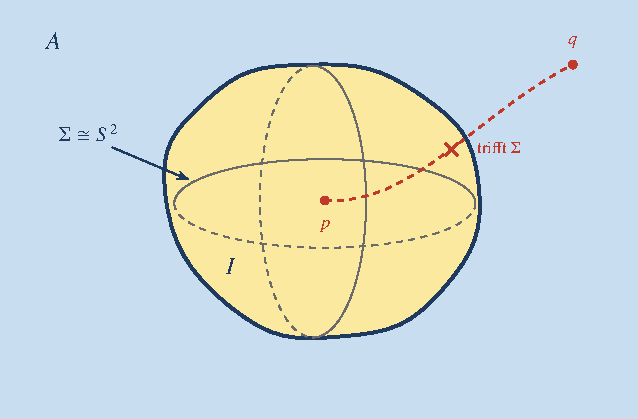
\includegraphics{papers/jordan/images/jordan_brouwer.pdf}
    \caption{Visualisierung des Jordan-Brouwer-Zerlegungssatzes im 3-dimensionalen Raum. $\mathbb{R}^{3}\setminus\Sigma$ zerfällt in genau zwei Komponenten: $\mathrm{I}$ beschränkt, $\mathrm{A}$ unbeschränkt}
\end{figure}

\begin{satz}[Jordan-Brouwer-Zerlegungssatz\label{jordan:satz:jordan_brouwer}]
    Sei $\Sigma \subset \mathbb{R}^{n}$ das Bild einer $C^1$-Einbettung von $(n-1)$. Dann gilt: \begin{enumerate}
        \item $S^n \setminus \Sigma$ besteht aus genau zwei Zusammenhangskomponenten.
        \item $\Sigma$ ist der Rand jeder dieser Komponenten.
    \end{enumerate} 
\end{satz}

Wie schon der originale Satz von Jordan, wirkt auch der Jordan-Brouwer-Zerlegungs\-satz auf den ersten Blick trivial, und genauso liegt die Schwierigkeit in der Allgemeinheit der Aussage.
Die eingebettete Linie kann eine beliebige Form annehmen und zusätzlich in beliebig vielen Dimensionen eingebettet werden.

Auch James W. Alexander selbst zeigte die potentielle Komplexität dieser Aussage, indem er 1924 die berühmte ``Gehörnte Sphäre'', konstruierte.
Sie trennt den Raum in zwei Teile, wie vom Satz von Jordan-Brouwer verlangt, aber das Äussere ist kein einfaches Komplement einer Kugel.
Es enthält eine unendliche Anzahl von Spitzen, die in den Raum hineinragen und Schleifen bilden, die sich nicht zusammenziehen lassen.

Während der Jordan-Brouwer-Zerlegungssatz sagt, wie viele Gebiete eine eingebettete Kreislinie erzeugt, sagt er jedoch nichts über die exakte Form dieser Gebiete aus.
Der Satz von Schoenflies liefert diese Information.

\begin{satz}[Der Satz von Schoenflies\label{jordan:satz:schoenflies}]
    Sei $\Sigma \subset \mathbb{R}^{2}$ eine geschlossene Jordan-Kurve und $S^1 \subset \mathbb{R}^{2}$ der Einheitskreis. 
    Dann ist der Homöomorphismus $h\colon \Sigma\to S^1$ zu einem Homöomorphismus $H\colon \mathbb{R}^2  \to \mathbb{R}^2$ erweiterbar.
\end{satz}

Veranschaulichen lässt sich der Satz von Schoenflies mit einem einfachen Gedankenexperiment: Man nehme eine beliebige Jordan-Kurve $\Sigma$ und befestige sie auf einem dehnbaren Tuch.
Man kann das Tuch nun so dehnen, dass die Kurve $\Sigma$ auf den Einheitskreis $S^1$ abgebildet wird.
Dies gilt für sämtliche $\Sigma$, egal wie wild sie auch sein mag.

Während dieser Satz für $n=2$ gilt, ist er für $n>2$ nicht mehr gültig, da es in höheren Dimensionen möglich ist, dass die eingebettete Sphäre $\Sigma$ eine Form annimmt, die nicht homöomorph auf eine Standard-Sphäre ist.
Trotz dieser Einschränkung bietet der Satz von Schoenflies eine Erweiterung des Satzes von Jordan auf eine höhere Dimension.

\subsection{Die Alexander-Dualität
\label{jordan:subsection:alexander}}

Mit der Alexander-Dualität haben wir das Ende unserer Reise zur Verallgemeinerung des Satzes von Jordan erreicht.
Sie liefert eine Verallgemeinerung des Satzes von Jordan auf beliebige Dimensionen und beliebige topologische Räume.

Um vom Jordan-Brouwer-Zerlegungssatz zur Alexander-Dualität zu gelangen, müssen wir einige Fragen, die wir beantworten möchten, aus einer allgemeineren Perspektive betrachten.
Die Frage ``In wie viele Teile zerlegt die Jordan-Kurve den Raum, in welchen sie eingebettet ist?'' muss als Spezialfall einer viel allgemeineren Frage betrachtet werden: ``Wie viele Löcher entstehen in welchen Dimensionen?''

\subsubsection{Löcher in der Topologie}

In der Topologie beschreibt das Konzept eines Lochs, mit welcher Art von geschlossenem Gebilde es umschlossen werden kann.
Die Dimension eines Lochs ist dabei die Dimension des umschliessenden Gebildes.

Das Konzept von Löchern erstreckt sich über beliebige Dimensionen, jedoch sind Löcher in Dimensionen $n>2$ schwer vorstellbar.
Löcher in den Dimensionen $n=0,1,2$ lassen sich jedoch leicht beschreiben:

\begin{itemize}
    \item \textbf{Löcher in Dimension 0: Lücken zwischen Teilen.} Das einfachste geschlossene Gebilde ist ein Paar von Punkten. Ist der Wegzusammenhang zwischen den Punkten unterbrochen, sind die Punkte in verschiedenen Komponenten. Zwischen ihnen liegt also ein Loch.
    \item \textbf{Löcher in Dimension 1: Tunnel.} Man nehme als Gebilde eine Schleife. Wenn sich diese Schleife innerhalb des Raumes nicht zusammenziehen lässt, hat sie ein Loch in Dimension 1. Bekannte Beispiele beinhalten den Kreis mit einem Loch im Inneren oder ein Bretzel, welcher von oben betrachtet wird, mit drei Löchern.
    \item \textbf{Löcher in Dimension 2: Hohlräume.} Ein Loch in Dimension 2 ist ein Hohlraum, der von einer geschlossenen Fläche umschlossen wird. Ein Tennisball hat ein Loch in Dimension 2, während eine Billiardskugel nicht hohl ist und entsprechend kein Loch in Dimension 2 hat.
\end{itemize}

Auf den ersten Blick scheint die Höhe der Dimension, welche ein Loch beschreibt, etwas unintuitiv.
So erwartet man, dass ein Loch in Dimension 1 durch ein 1-dimensionales Gebilde beschrieben wird.
Doch das Loch selbst ist nicht das Gebilde, sondern der Raum, der von diesem Gebilde umschlossen wird, und dieser Raum ist in der Dimension um eins höher als das Gebilde selbst.

Im Kontext des Satzes von Jordan betrachten wir die Jordan-Kurve $\gamma$ als ein geschlossenes Gebilde, das den Raum in zwei Teile trennt.
Jordan-Brouwer betrachet dabei nur eine einzelne Dimension.
Die Frage ``In wie viele Teile zerlegt die Jordan-Kurve den Raum, in welchen sie eingebettet ist?'' betrifft nur die 0-dimensionalen Löcher des Komplements.

\subsubsection{Betti-Zahlen}
\index{Betti-Zahl}%

Die Betti-Zahlen $b_i$ zählen die Anzahl der unabhängigen Löcher in Dimension $i$.
Unabhängigkeit bedeutet hierbei, dass die Löcher nicht durch andere Löcher erzeugt werden können.
Man nehme zum Beispiel die Form der Zahl 8: Grundsätzlich besteht sie aus zwei Kreisen, die sich in der Mitte berühren.
Es gibt drei offensichtliche Schleifen: Die obere, die untere und eine, die beide nacheinander durchläuft.
Trotzdem ist die Betti-Zahl $b_1$ nur 2, da die dritte Schleife durch die beiden anderen erzeugt werden kann.

\subsubsection{Homologie und Kohomologie}

Um die Alexander-Dualität nachvollziehen zu können, müssen wir erst mit den Begriffen der Homologie und Kohomologie vertraut werden.
Dabei ist zu beachten, dass die nachfolgende Einführung der Veranschaulichung der Konzepte dient und keine vollständige Definition dieser hochabstrakten Konzepte darstellt.

Die Homologie ist ein Werkzeug, welches uns erlaubt, Löcher in beliebigen Dimensionen zu zählen.
\index{Homologie}%
Man zerlegt den Raum in eine endliche Anzahl von einfachen Gebilden, die als Simplizes bezeichnet werden.
Eine Kette ist eine endliche Summe von Simplizes der gleichen Dimension, zum Beispiel eine Menge von Kanten, die zusammen einen Weg bilden.
Jede Kette hat einen Rand, der aus Simplizes der nächstniedrigeren Dimension besteht.
So ist beispielsweise der Rand einer Fläche eine Kette von Kanten, die die Fläche umschliessen.
Eine Kette ohne Rand heisst Zyklus und wird auch als geschlossene Kette bezeichnet.
Beispiele hierfür sind Schleifen ohne Enden oder Hüllen ohne offene Stellen.
Hierbei wird modulo $2$ gerechnet: Wird eine Kante zwei mal in einem Zyklus verwendet, hebt sie sich auf.
Legt man zwei benachbarte Dreiecke zusammen, so hebt sich die gemeinsame Kante auf, und es bleibt nur der Rand des neu entstandenen Vierecks.
Zyklen, welche als Ränder eines höherdimensionalen Gebildes auftreten sind trivial, da sie kein Loch umschliessen.
Die Homologie ist die Menge aller Zyklen, welche nicht Ränder sind.

Die Kohomologie verwendet die gleichen Konzepte, jedoch in umgekehrter Richtung.
\index{Kohomologie}%
Statt Objekte in den Raum zu legen, definiert man Messvorschriften, welche die Objekte im Raum messen.
Jedem Baustein des Raumes wird ein Wert zugeordnet, und die Summe der Werte über eine Kette ist der Wert der Kette.
Ein einfach verständliches Beispiel ist eine sogenannte Mautstelle.
Man stelle sich ein Torus vor, auf welchem eine Linie quer über den Schlauch gezogen wird.
modulo $2$ zählt nur, ob die Anzahl gerade oder ungerade ist.
Verschiebt man die Schleife, ändert sich die Anzahl der Schnittpunkte, aber die Parität bleibt erhalten.
Eine neue Kreuzung entsteht immer zusammen mit einer zweiten.
Eine Schleife, die sich um den Torus windet, kann nicht auf eine Schleife ohne Kreuzung deformiert werden.

Wie bei der Homologie benötigen wir zwei Filter.
Konsistente Messungen, auch Kozyklen genannt, sind Messvorschriften, die auf jedem Rand null ergeben.
Nur dann kann man sicherstellen, dass die Messung nur auf das Loch reagiert, und nicht auf den Rand.
Triviale Messungen, auch Koränder genannt, sind Messvorschriften, die aus einem Potential, aus Höhendifferenzen einer Höhenfunktion, abgeleitet werden können.
Eine solche Messung ergibt auf jeder geschlossenen Schleife null, weil man am Ende wieder auf derselben Höhe ist.
Entsprechend kann sie nicht auf ein Loch reagieren.
Die Kohomologie ist die Menge aller Kozyklen, welche nicht Koränder sind.

\subsubsection{Alexanders Beweis}

\begin{satz}[Der Satz von Alexander\label{jordan:satz:alexander}]
    Sei $G$ eine abelsche Gruppe und sei $X \subset S^n$ eine kompakte,
    nichtleere, echte Teilmenge, die lokal zusammenziehbar ist.
    Dann gilt für alle $i$:
    \[
        \tilde{H}_i(S^n \setminus X; G) \cong \tilde{H}^{n-i-1}(X; G).
    \]
\end{satz}

Der Satz ist eine Aussage über die Isomorphie von Gruppen:
Er verbindet die Homologie des Komplements $S^n \setminus X$ mit der Kohomologie von $X$.

Für einen Raum $Y$ bezeichnet
\[
    \tilde{b}_k(Y) := \dim_{\mathbb{Q}} \tilde{H}_k(Y; \mathbb{Q})
\]
die $k$-te \emph{reduzierte} Betti-Zahl.
Sie stimmt mit der gewöhnlichen Betti-Zahl $b_k(Y)$ überein, außer für
$k = 0$: Dort gilt $\tilde{b}_0(Y) = b_0(Y) - 1$.

Um aus dem Satz eine Aussage über Betti-Zahlen zu gewinnen, ist noch ein
weiterer, nicht ganz einfacher Schritt nötig.
Zum einen wählt man als Koeffizienten einen Körper, etwa $\mathbb{Q}$.
Dann sind beide Seiten Vektorräume, und aus ihrer Isomorphie folgt die Gleichheit ihrer Dimensionen.
Zum anderen sind die Betti-Zahlen über die Homologie definiert, auf der rechten Seite steht jedoch die Kohomologie.
Dass Homologie und Kohomologie mit Körperkoeffizienten dieselbe Dimension haben, folgt aus der Dualität zwischen Homologie und Kohomologie, dem sogenannten universellen Koeffiziententheorem.

Zusammen ergibt sich:

\begin{korollar}[Alexander-Dualität für Betti-Zahlen]\label{jordan:korollar:alexander}
    Sei $X \subset S^n$ wie im Satz~\ref{jordan:satz:alexander}.
    Dann ist für alle $i$ die $i$-te reduzierte Betti-Zahl des
    Komplements $S^n \setminus X$ gleich der $(n-i-1)$-ten reduzierten
    Betti-Zahl von $X$:
    \[
        \tilde{b}_i(S^n \setminus X) = \tilde{b}_{n-i-1}(X).
    \]
\end{korollar}


Es besteht also eine Dualität zwischen den ``Löchern'' des Komplements und denen von $X$ in komplementären Dimensionen.
Der Satz von Jordan ergibt sich daraus als Spezialfall.
Ist $X$ homöomorph zu $S^{n-1}$, so liefert das Korollar für $i = 0$
\[
    \tilde{b}_0(S^n \setminus X) = \tilde{b}_{n-1}(S^{n-1}) = 1.
\]
Da die reduzierte nullte Betti-Zahl um eins kleiner ist als die Anzahl der Zusammenhangskomponenten, zerfällt $S^n \setminus X$ in genau zwei Komponenten.
Für $n = 2$ ist dies gerade die Zerlegungsaussage des Satzes von Jordan.
Der Satz von Alexander verallgemeinert diese also auf beliebige Dimensionen und auf beliebige kompakte, lokal zusammenziehbare Teilmengen der $S^n$.
